\section{CIG: Computational\\ Intelligence in Games}\label{subsecCIG}

% co-exists with CIG conference
% games are run privately on several computers just before the conference  
The CIG StarCraft RTS AI Competition is a part of the program of the IEEE Computational Intelligence in Games (CIG) conference since August 2010. 
% Changes on CIG StarCraft AI Competition (Organizers, Tournament Software, Rules (Maps), Open Source Policy
Similarly to AIIDE competition, all the bot games are run separately on several computers prior to the conference and the results are then announced during the event. 
% We planed to use a single machine using virtual machines in this year. But, we don't have enough time to confirm that it has no concern on the correctness of the results. 
Unlike in AIIDE and SSCAIT, the map pool of the CIG competition is not known in advance for the competitors. Also, the CIG competition no longer enforces an open source code requirement to compete.
% Those rules have been changed 
% Insert the figures from the CIG 2017 presentation 
% Cite 2016 on CIG 2016 competition published in AI Magazine Paper 

\subsection*{CIG 2016-17 Updates \& News}\label{subsecCIGnews}

% CIG 2017 scheduled for Summer 2017
% CIG 2016 happened in Sept. 2016.  
CIG 2017 is scheduled to happen in New York City, USA on late August 2017, which is just after the submission deadline of this paper. Therefore, we will report on CIG 2016, which happened on September 2016. 

% two round-robin stages: qualifying stage and final stage. half of Q goes to F
% persistent files are erased between stages 
% qualif. stage: 11988 games with 16 bots
% final stage: 2799 games with 8 bots
% ran for 8 days on 17 computers
% winner: tscmoo by Vegard Mella from Norway

The 2016 installment of CIG competition hosted {\em 16 participants}, out of which 9 were new or updated bots and 7 were re-entries from previous year. CIG 2016 competition was divided into two stages: The {\em Qualifying} stage and the {\em Final} stage. The first qualifying stage consisted of Round Robin tournament between all 16 participating bots. In total, 11988 games were played in this stage. After the qualifying stage, best 8 bots were selected to proceed to the final stage: {\em tscmoo, IronBot, LetaBot, ZZZbot, Overkill, UAlbertaBot, MegaBot} and {\em Aiur}.

All the persistent files accumulated by the bots in the qualifying stage were deleted before entering the finals. This stage consisted of 2799 Round Robin games between the 8 bots. All the games ran on 17 computers for 8 days. The winner of the final stage, {\em tscmoo} bot created by Vegard Mella from Norway, was announced the overall winner of CIG 2016 tournament with 456 wins and $65.14\%$ win rate in the final stage. Detailed results are depicted in Figure~\ref{figCIGresults}. 

% Post-Confererence Event (Man vs. Human Match) 
After this year competition, Sejong University organized special event matches between human players and StarCraft AI players at 31st Oct 2017. In the match, our university invited one novice player (ladder rating around 1100), one middle-level player (around 1500), and professional gamer, Byung-Gu Song. For the AI side, it included ZZZKBOT, the winner of CIG 2017 competition, TSCMOO, 2nd ranker in CIG, and MJBOT, specially designed AI for human players. The MJBOT has been developed since June 2017 by Cognition Intelligence Laboratory (leaded by Kyung-Joong Kim) to beat novice/middle-level players. 

In the event match, each human player had a single match against the AI players. In total, there were nine matches (3 human players X 3 AI players). In the first match, the novice human player won the first game against MJBOT but lost two games against ZZZKBOT, and TSCMOO. Although MJBOT lost the first game, it's nearly close to the win of the MJBOT but fail to finalize the match because of the programming bug. In the next session, the middle-level human player lost all the three games against the AI players. However, the Byung-Gu Song, a professional player won the all three games. It means that the AI players have potential to compete against novice and middle-level players, but not yet to the professional gamers. You can find the results and replay files of the matches from the website \footnote{\url{https://cilab.sejong.ac.kr/}}. 

% Cite our work on Human Evaluation? 

\begin{figure}[h]
  \centering
  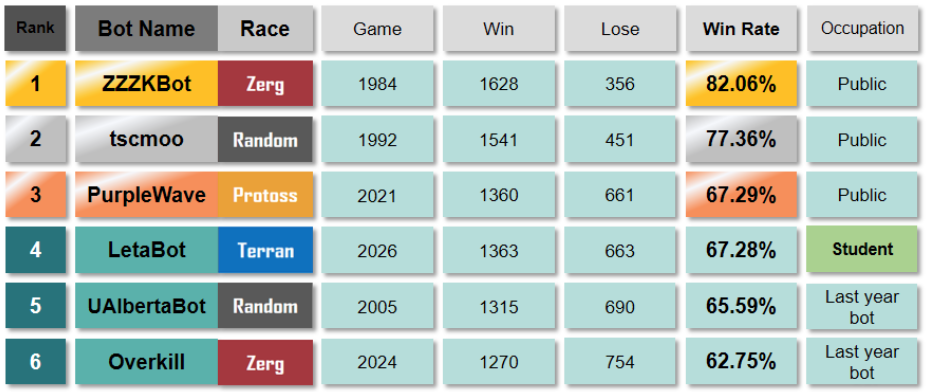
\includegraphics[width=0.5\textwidth]{fig/cig-results.png}
  \caption{Detailed results of the CIG 2016 competition final stage.}
  \label{figCIGresults}
\end{figure}

\begin{figure}[h]
  \centering
  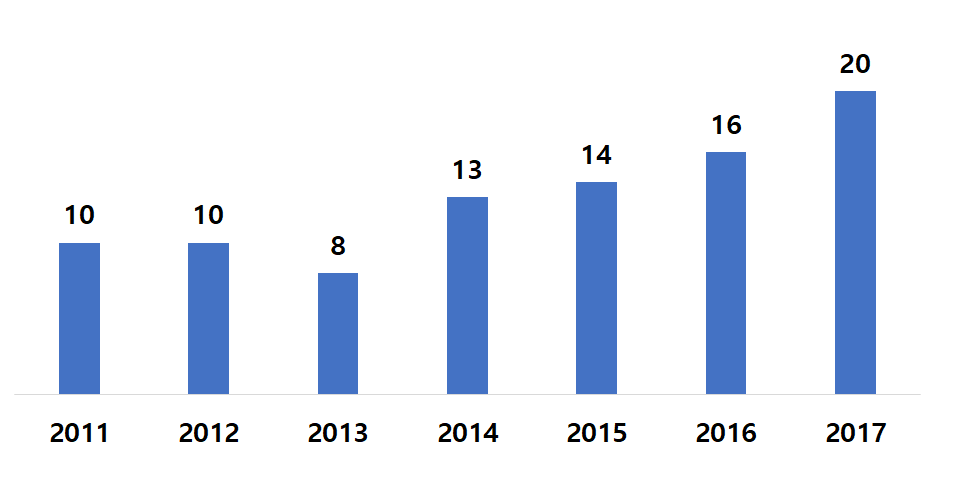
\includegraphics[width=0.5\textwidth]{fig/cig-num_of_submissions.png}
  \caption{The number of submissions in CIG StarCraft AI Competition.}
  \label{figureCIGsubmissions}
\end{figure} 


\begin{figure}[h]
  \centering
  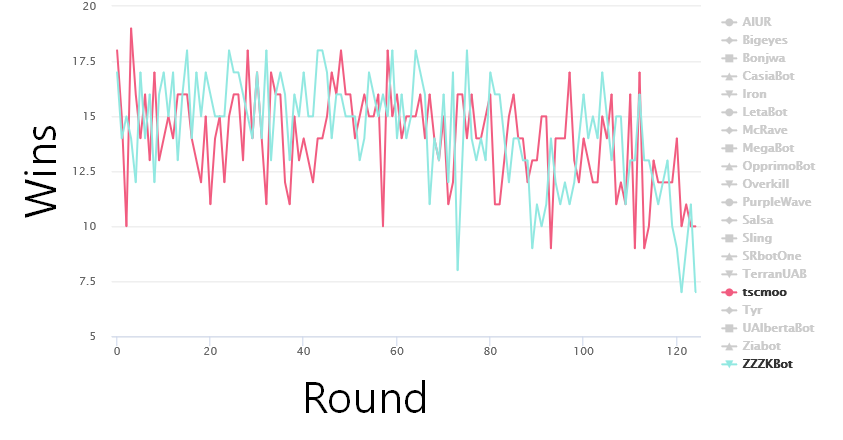
\includegraphics[width=0.5\textwidth]{fig/cig-tscmoo-zzzkbot-winrate.png}
  \caption{The change of wins over multiple rounds for ZZZKBot (1st ranker), and TSCMOO (2nd ranker).}
  \label{figureCIGZZZTSCMOO}
\end{figure} 

\begin{figure}[h]
  \centering
  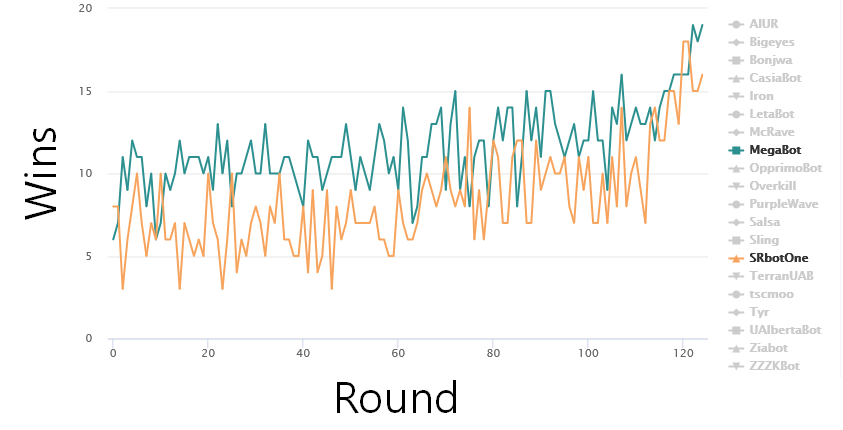
\includegraphics[width=0.5\textwidth]{fig/cig-megabot-srbotone.png}
  \caption{The change of wins over multiple rounds for MegaBot and SRBotOne.}
  \label{figureCIGZZZTSCMOO}
\end{figure} 

\begin{figure}[h]
  \centering
  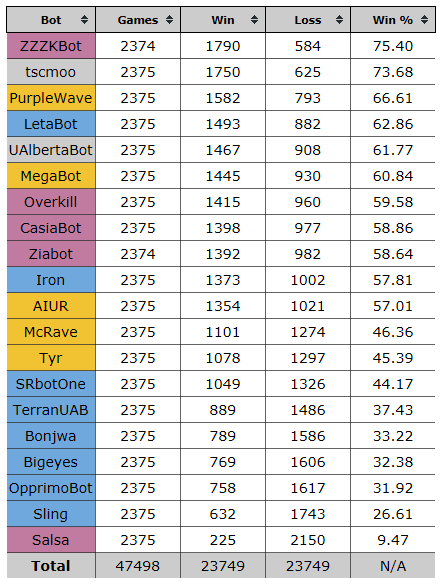
\includegraphics[width=0.5\textwidth]{fig/cig2017.png}
  \caption{The win rate of CIG 2017 competition entries.}
  \label{figureCIG2017}
\end{figure} 

